\chapter{Describing Machine Learning Approaches}

\section{Machine Learning}

Machine learning has become a very popular topic in recent years due to the sheer amount of data that has to be processed.  Not only does this large amount of data need more advanced and intelligent ways to dealing with it, but there is also a huge incentive to do so.  By using machine learning techniques additional meaning and patterns can be extracted from the data and conclusions can be drawn from it. % cite data manag systems 
Machine learning is often applied to data mining tasks, looking at data and decerning information from it, in this case the data being mined is the large amount of web requests.

This has numerous benefits when applied to a security application such as web threat detection.  Primarly it allows the system to have some sort of feedback mechanicism to improve its detection and perhaps even prevention.  A system that is unable to learn overtime will not be able to overcome new techniques designed to evade the current detection systems unless it is manually updated.  And as discussed before, manual updating is not only a very inefficient time consuming task, but it is becoming infeasible with the growth of these attacks.  Identifying patterns from data itself is very useful when the fact that many of the attacks follow some kind of a basic syntax or format, while there are many ways to evade detection typically a common method and intent for the attack to be done.

The way machine learning operates is by identifying a series of features in the data set in question, the features can be classified as continuous, categorical or binary.  These features are used by the algorithm to learn and to make decisions, the key distinction about machine learning is it is not told what to do but instead is allowed to make its decision based on measurements such as performance.   %cite supervised machine learning
  
\subsection{Supervised Learning}

Machine learning algorithms can either use supervised learning or unsupervised learning.  In supervised learning the system is provided with labelled data, data that states what the end result should be so the system can be accurately trained from the beginning.  There is also another type of learning called reinforcement learning where an external source informs the system how well it is working or not.

Supervised learning has its issues that have to be overcome however, the first of which being collecting the original data set.  If there is prior research or people in the know that can suggest what features to use than the process is more trivial, however if not then this is often identified using a brute force method.  The problem with using a brute force method other than the complexity is that the data has the potential to be noisy and missing important features which can lead to further problems.  Learning from extremely large datasets is very inefficient and slow as well, therefore it is often desired to minimize the data set while still maintaining the performance of the system; this process is referred to as instance selection.  Lastly, having a large amount of features in your data set can also increase the complexity of the system.  To solve this, irrelevant and redundant features should be removed but if many of the features depend on each other and cant be removed this can lead to inaccuracy from the results of the learning.  In order to remedy this, new features can be constructed or altered that are more concise or accurate which can improve the entire system as a whole.

One of the biggest steps in creating a machine learning system is selecting the right algorithm for the dataset, each which their own advantages, disadvantages and times where they are applicable (Section \ref{sec:genDisadvantages}, \ref{sec:svmDisadvantages}). 

\section{Genetic Algorithm}

A genetic algorithm is a search-based algorithm that makes use of the mechanism of machine learning in order to locate optimal or near-optimal solutions.  This is what is meant by the term 'search' that is used in other algorithms such as local search, or simulated annealing, it is not about locating something from a particular data set but rather searching for the best possible answer.  Such algorithms, especially in the case of a genetic algorithm use fitness functions and reward systems to distinguish between a better solution and one that should not be considered anymore.  % search based software engineering

As the name suggests, a genetic algorithm mimics how genetic development in the real world works and how species improve over time.  The algorithm begins with an initial population of individuals, an individual is a possible solution to the problem in question.  This initial population has it's fitness evaluated using some form of calculation tailored to suit the problem; for our purposes for web threat detection the fitness will be evaluated as the following:

\begin{algorithm}[H]
	\setstretch{1.0}
	\label{alg:fitness}
	\caption{Fitness algorithm for use in genetic algorithm}
	
	$\alpha \leftarrow The\ number\ of\ possible\ correct\ detections$ \\
	$\beta \leftarrow The\ number\ of\ possible\ incorrect\ detections$ \\
	$\gamma \leftarrow The\ number\ of\ possible\ false\ positives$ \\

	$fitness \leftarrow \frac{correct\ detections}{\alpha}\ - \frac{false\ positives}{\gamma}\ - \frac{incorrect\ detections}{\beta \cdot 8}$
\end{algorithm}

Correct detections improve the fitness of a particular individual and it is more likely to be selected for genetic operators later on, where as false positives and incorrect detections impact the fitness negatively with incorrect detections having less of an impact than the former.  For example, if we are looking for SQL injections, every request that is a SQL injection that is detected is correct, if it identifies a request that isnt an attack at all as a SQL injection then it is a false positive and if it identifies an XSS or RFI attack as an SQL injection, then this is incorrect.

In order for the genetic algorithm to produce a new population it makes use of what are called genetic operators which commonly include performing crossovers and mutations.  Two individuals at a time in the population are selected by a selection algorithm and first crossed over, there are many ways to perform a crossover but a single-point crossover will be used for this research.  A position is selected to perform the crossover, this is referred to as a locus, for our purposes this refers to selecting a segment, this segment is then swapped with the other selected individual to produce two individuals with unique chromosomes, or in other words a different configuration.  This continues until the algorithm has produced enough new individuals to fill the population, in addition, at the beginning of this process it is possible to mark some of the top individuals as elite and preserve them over to the new population.  Before continuing to the next iteration every single allele, or piece of information, in each individual has the small potential to be mutated this is what causes the population to have diversity.  This process then repeats many times, each time being referred to as a generation and by the end of the process there should be a set of individuals that are closer to solving the problem.

\subsection{Current Genetic Algorithm Solutions}

These genetic algorithm techniques have been applied to web threat detection already, one particular paper focused on using various variants of an attack to detect network related attacks.  While they may not have directly used a genetic algorithm in their solution, the core idea is very similar to how a genetic algorithm operates in generating different individuals and seeing if they perform better.  These exploit variants were used to test signatures based detection methods to see if it was possible to evade them and results showed that it was.  This is proof that traditional models for detection cannot be made absolutely perfect and that the technique of using genetic algorithm technniques is atleast worthwhile for evading detection. % cite testing network based instrusion 

As of recently however, research has taken this idea and done the opposite, using a genetic algorithm directly to detect web attacks rather than evade detection.  This was done by using the genetic algorithm to make variants of attack signatures that best detect SQL injections, XSS, and RFI attacks through the text-based web request logs.  The results of which were very promising with around a 90\% detection accuracy reported which exceeded a traditional regular expression signature based detection system. % cite main paper

For this research, this recent research is the starting point for improving the genetic algorithm approach and gathering more detailed results about its function, as well as the comparison point to another machine learning technique, support vector machines.

\section{Support Vector Machine}

A support vector machine's main technique for classifying data is by dividing the data set in two or more categories with the largest margin between the seperation(s), referred to as a hyperplane(s).  The point in maximizing this buffer between the two data sets is to reduce the chances of error as much as possible.  Once this hyperplane is computed, points that lie within the margin are referred to as support vectors, hence the name, and it is these points which were what calculated the hyperplane in the first place, the other data points were ignored (Figure \ref{fig:svmmargin}).  

\begin{figure}
	\label{fig:svmmargin}
	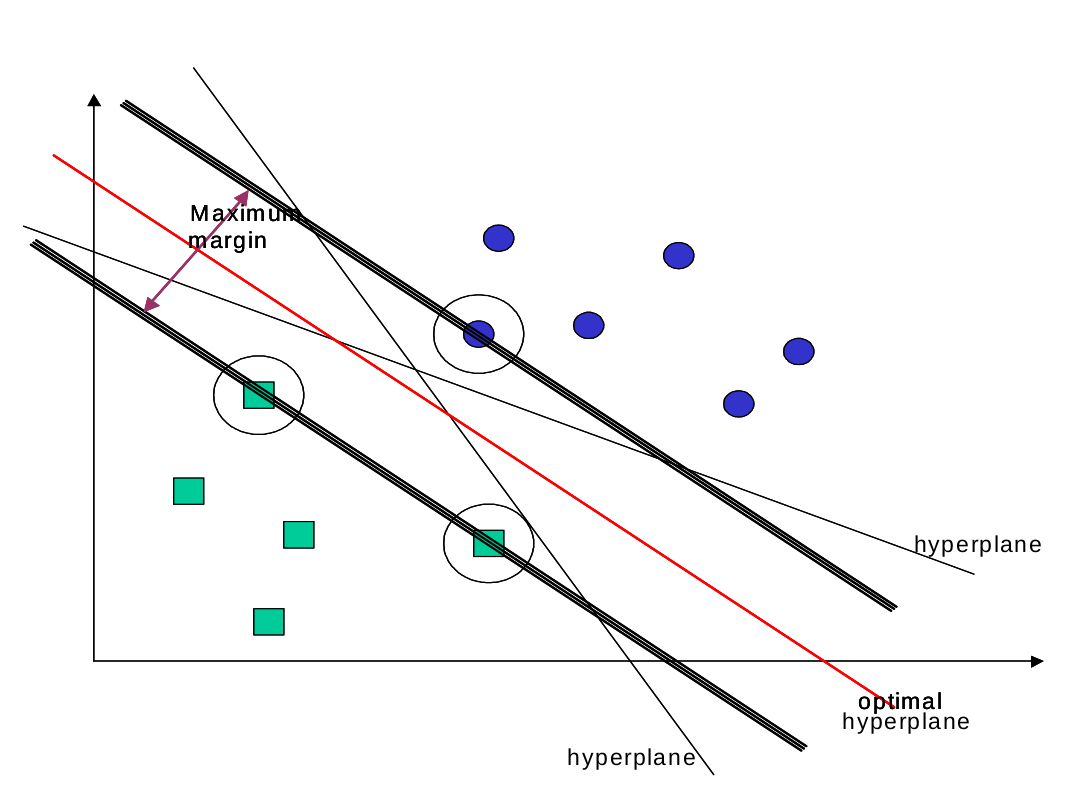
\includegraphics[width=450px]{./assets/img/svmmargin.png}
	\caption{Example of a linear seperated SVM}
\end{figure}

The fact that the SVM is determined by the support vectors which is usually a very small subset is great because it means that the speed does not significantly slow down with a larger amount of features.  However it is very realistic to imagine data that cannot be easily divided and so soft margins that allow for misclassifications and in worse cases the data can be mapped in a higher dimensional space to open up other options.  This higher dimensional space is referred to as the transformed feature space, however it makes simple linear seperations in the higher dimensional space transform into non-linear seperations when you return back from the higher dimension.  

If this feature space data is mapped to Hilbert space, referred to with $\Phi$, which allows for traditional vector calculations to be extended to many dimensions using dot products using equations in the form of: $\Phi\left(x_i \right)\cdot\Phi\left(x_j \right)$.  This means that we can use what is referred to as a kernel function to avoid ever having to determine the mapping to $\Phi$ and can calculate directly in feature space.  A kernel function is in the form of: $K(x_{i},x_{j}) = \Phi(x_i) \cdot \Phi(x_j)$. % cite supervised machine learning
There are many commonly used kernels, three of which will be used in this research: linear, polynomial (with degree 3), and radial basis function (Table \ref{tab:kernels}).  

\begin{table}[h]
	\centering
	\label{tab:kernels}
	\begin{tabular}{|p{1.5in}|p{4.5in}|}
	\hline
		\textbf{Kernel Function} & \textbf{Mathematical Formula}\\
	\hhline{|=|=|}
		Linear  & $K(x_{i},x_{j}) = \langle x_{i},x_{j}\rangle$ \\
	\hline
		Polynomial & $K(x_{i},x_{j}) = (\langle x_{i},x_{j}\rangle + 1)^d, d: degree$ \\
	\hline
		Radial Basis Function (RBF) & $K(x_{i},x_{j}) = \exp\left(\frac{- \parallel x_i - x_j \parallel^2}{2\sigma^2} /\right), \sigma : width\ of\ RBF\ function$ \\
	\hline
	\end{tabular}
	\caption{Kernels that will be used and their mathematical function} % cite instruction detection for cost based
\end{table}

Once the SVM is trained using the kernel method the only step is to pass in all of the testing data and see where on the graph it falls in order to classify it.  An SVM can at times get very computational intensive and can run very slow, this is often due to the choice of the kernel function choosen as well as the parameters that go into the kernel.  For example, a linear kernel is very simple where as an RBF kernel is much more complex.  Two parameters that are worth mentioning for the SVM training process are $\gamma$ (gamma) and C.

Gamma is used in the polynomial and RBF kernels to define how much influence each training vector has on the seperation.  A lower gamma value corresponds to a far influence, when gamma is too small the influence of any support vector may extend to the entire set and the end result would instead just be regions of high density being isolated from others.  On the converse if the gamma is too high then the influence would only be the support vector itself.  The C parameter is the penalty cost assocated with misclassification, if C is low then classification is more relaxed where as a higher C will encourage more support vectors to be choosen to achieve a more accurate result.  % cite rbf svm parameters
There is no way to know what are the best values to choose because it depends on the dataset in question so this must be done by doing testing.

\subsection{Current Support Vector Machine Solutions}

Support vector machines have also been applied to web threat detection as well but only in the lower layers of the OSI model dealing with network related attacks such as denial of service attacks.  One such study used a cost based support vector machine to detect web attacks and was able to detect them with an overall accuracy of 99\%.% cite intrusion detection system based on cost based
Likewise, another study compared the usage of an SVM versus an artificial neural network and found that the SVM was much faster in comparison along with achieving a 99\% accuracy as well.%cite intrusion detection using neural networks
These two studies shows that the SVM approach is a viable one and can be used for practical applications with web threats, so it will be interesting to see how well the algorithm preforms compared to the genetic algorithm approach for application layer attacks as well.


